\chapter{Asking Women Billionaires How They Got Rich!}

This lecture proceeds by misdirection. It begins with yachts, valuations, oil, and the word ``billionaire,'' but these are not yet explanations; they are lures. Only after the teaser collage does the lecture settle into its real method, which is to move from visible wealth to the machinery underneath it. What gives the chapter its mathematical weight is not a blackboard derivation, because there is none, but a sequence of clean numerical compressions: years in business, one-year earnings, deal size, phone-call rebuild claims, exit valuation, founder equity, an initial \(\$175{,}000\) turning into roughly \(\$100\) million in ten years, and finally a long-duration founder path measured not by one lucky break but by restart, ownership, and differentiation.

\section{Cold Open: Miami as a Wealth Field}

The lecture opens in montage. A yacht appears, then an oil-industry answer, then a 2023 sale, then a personal equity figure of roughly \(\$90\) million, and finally the host presses on the word ``billionaire.'' The order matters. We are not yet being taught. We are being made curious.

Only after that does the host reset the scene. He tells us that there are more than \(360\) female billionaires in the world,
\begin{equation}
N_{\text{female billionaires}} > 360,
\end{equation}
and he relocates the inquiry to Miami. This is not merely geography. The city becomes a field site in which luxury is treated as evidence to be interrogated rather than as an explanation in itself.

The lecture's method is already visible here. We begin from an object that everybody can see, but we do not stop there. The car, the yacht, the valet line, the district, these are only the outer shell. The real question is always: what business structure, what operating style, what relation to risk, leverage, and time produced the object in front of us?

\section{The Oil Entrepreneur: Rule-Breaking and the First Mechanics}

The first full case is the woman in the G-Wagon. The lecture introduces her in the usual visible way, through the car, but immediately narrows to industry, duration, and scale. She says she is in oil, that she has been a business owner for about sixteen years, and that the most money made in a single year was on the order of six to seven million dollars:
\begin{equation}
t_{\text{oil}} \approx 16\ \text{years},
\qquad
Y_{\text{oil}} \approx \$6\text{--}7\,\text{million}.
\end{equation}

\paragraph{Anecdote.}
The first financial advice she offers is not a spreadsheet rule but a social one: well-behaved women rarely make history. The point is not rebellion for its own sake. The point is that strict obedience to established paths rarely produces exceptional outcomes.

\paragraph{Claim.}
Boldness, in this lecture, is not romantic decoration. It is a business disposition. The operator must be willing to move where permission is unclear, where conventional behavior would have stopped.

\paragraph{Mechanism.}
The lecture then refuses to leave the idea at the level of posture. It asks what business actually made the money. Her answer is not singular: manufacturing solar panels and pumping crude oil. Then it asks about the largest deal, and the figure settles at roughly
\begin{equation}
D_{\text{max,oil}} \approx \$28\,\text{million}.
\end{equation}
The earlier \(\$20\) million number should be read as conversational refinement rather than as a competing stable datum.

This is the first place where the lecture becomes operational. The entrepreneur does not describe wealth as an aura. She describes it as deal-making inside a sector, and then even more narrowly as selling. She says she sells, sells, sells. She roots this not only in bravado but in long experience with people through customer service.

\subsection{Question \& Answer}

\paragraph{Question.}
How does boldness become business method rather than merely attitude?

\paragraph{Answer.}
The lecture's answer is that boldness must cash out as repeated commercial action. The aphorism about rule-breaking is not allowed to float free. It is immediately tied to a concrete industry, a concrete duration in that industry, a concrete earnings range, and a concrete deal size. In other words, boldness becomes serious only when it is attached to a market, a sale, and a number.

\section{Sales, Borrowed Capital, Network, and the Tax-Team Shell}

The oil case continues by moving from selling to capital handling. She is asked whether she borrows from banks, and she says yes, all the time. Then comes the lecture's schematic leverage rule:
\begin{equation}
B
\to
\text{spread across uses}
\to
\text{multiplied returns}
\to
\text{repayment}.
\end{equation}
We should keep this as a compact reconstruction of the spoken logic, not as a literal finance model with stated rates, maturities, or cash-flow schedules. The lecture gives us sequence, not underwriting.

\paragraph{Anecdote.}
Her language is quick and compressed. She spreads the money out, budgets it, multiplies it, and often pays it back before it has even fully made what it was meant to make. Whether every step of that statement would survive forensic scrutiny is not the point at this stage. The lecture is teaching a style: money enters as borrowed fuel and is not left as a static lump.

\paragraph{Claim.}
Leverage here is less about debt worship than about motion. Money must circulate through uses rather than remain inert.

\paragraph{Mechanism.}
The next compression is even harsher. If she lost everything tomorrow, she says she could make it back in ten phone calls:
\begin{equation}
n_{\text{calls}} = 10.
\end{equation}
This is almost certainly rhetorical in the narrow sense, but the structural lesson is clear: once a network is real, it becomes a reserve asset. Social capital is not a metaphor in this lecture. It is rebuild capacity.

The lecture then widens from network to the shell around money. She speaks of trust accounts, write-offs, portfolios, and a very strong financial team. The advice is not subtle: invest in the best advisors, the best tax attorneys, the best financial operators, because a good team makes money for you, even in your sleep. That phrase should not be over-literalized, but the mechanism is plain enough. Wealth is preserved not only by what we own, but by the technical architecture through which it is held and administered.

\begin{figure}[h]
\centering
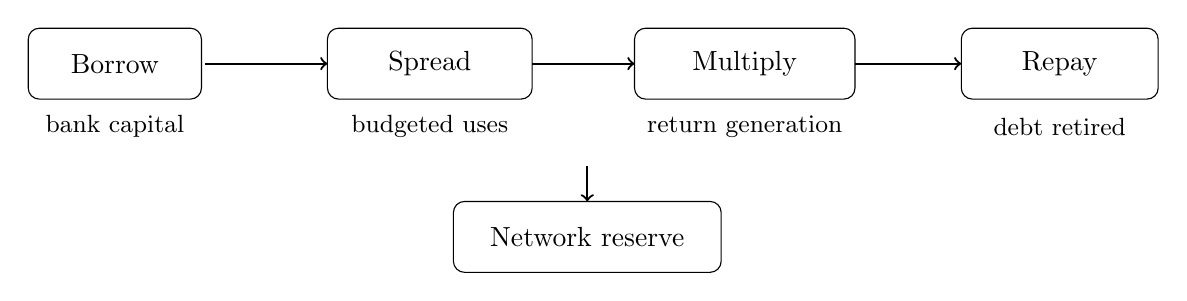
\begin{tikzpicture}[scale=1]
\node[draw, rounded corners, minimum width=2.2cm, minimum height=0.9cm] at (0,0) (a) {Borrow};
\node[draw, rounded corners, minimum width=2.6cm, minimum height=0.9cm] at (4,0) (b) {Spread};
\node[draw, rounded corners, minimum width=2.8cm, minimum height=0.9cm] at (8,0) (c) {Multiply};
\node[draw, rounded corners, minimum width=2.5cm, minimum height=0.9cm] at (12,0) (d) {Repay};

\draw[->, thick] (1.15,0) -- (2.7,0);
\draw[->, thick] (5.3,0) -- (6.6,0);
\draw[->, thick] (9.4,0) -- (10.75,0);

\node[draw, rounded corners, minimum width=3.4cm, minimum height=0.9cm] at (6,-2.2) (e) {Network reserve};
\draw[->, thick] (6,-1.3) -- (6,-1.75);

\node at (0,-0.8) {\small bank capital};
\node at (4,-0.8) {\small budgeted uses};
\node at (8,-0.8) {\small return generation};
\node at (12,-0.8) {\small debt retired};
\end{tikzpicture}
\caption{Transcript-based reconstruction of the first entrepreneur's operating sequence. The lecture presents borrowing, distribution of capital, multiplication, and repayment as a process rather than as a single investment event, with network functioning as a latent reserve.}
\end{figure}

\subsection{Question \& Answer}

\paragraph{Question.}
When does leverage help, and when is the deeper leverage actually the team around the money?

\paragraph{Answer.}
The lecture gives a two-layer answer. Borrowed money helps when it is moved intelligently through uses and brought back under control. But the more durable leverage appears one level higher: the network that can restart the machine, and the advisory shell that keeps wealth from leaking away through bad structure, bad tax handling, or weak administration. Debt can accelerate a machine. The right team determines whether the machine survives.

At the end of this case the host pauses to widen the lesson. Oil is not a sector most viewers instinctively expect from a woman stepping out of a G-Wagon in Miami. That is precisely why the recap matters. Money is being made in more places than the naive imagination allows.

\section{The Solidcore Case: From \(\$175{,}000\) to \(\$100\) Million}

The second major case begins, again, with a visible object, now a baby-blue Bentley. But this section quickly becomes the chapter's numerical center of gravity. The entrepreneur explains that she sold her company in 2023. Her personal equity at exit was worth about \(\$90\) million, while the company itself was valued at a little over \(\$300\) million:
\begin{equation}
E_{\text{exit}} \approx \$90\,\text{million},
\qquad
V_{\text{company}} > \$300\,\text{million}.
\end{equation}
The transcript briefly blurs million and billion in the host's repetitions, but the internal scale makes clear that millions are intended.

A rough ownership fraction is therefore
\begin{equation}
f_{\text{equity}}
\approx
\frac{E_{\text{exit}}}{V_{\text{company}}}
\approx
0.30.
\end{equation}
This should be read cautiously, because the denominator is only specified as a little above \(\$300\) million.

Then comes the lecture's sharpest mathematical compression. She says that she put \(\$175{,}000\) into Solidcore and that it turned into roughly \(\$100\) million in ten years:
\begin{equation}
I_0=\$175{,}000,
\qquad
V_{10}\approx \$100\,\text{million}.
\end{equation}

\paragraph{Anecdote.}
This is where the lecture abruptly stops being merely a parade of large exits. We now have an initial amount, a final amount, and a time horizon. That is enough to ask a real quantitative question.

\paragraph{Claim.}
Her explicit doctrine is that, for an entrepreneur who genuinely has the special sauce, the best early investment is often the self. Later, after the big win, she moves into preservation mode and diversifies through startups, private equity, hedge funds, the stock market, and loans. But the lecture insists that the first move is concentration, not diversification.

\paragraph{Mechanism.}
The numerical story can be compressed in two ways. First, by simple multiple:
\begin{align}
M
&=
\frac{V_{10}}{I_0}
=
\frac{100{,}000{,}000}{175{,}000}
\approx 571.4.
\end{align}
Second, if we want a start-end equivalent annual growth rate,
\begin{align}
r_{\text{eq}}
&=
\left(\frac{V_{10}}{I_0}\right)^{1/10}-1
\approx 0.887.
\end{align}
So the start-end story, collapsed into a single annualized number, corresponds to about \(88.7\%\) per year. We should be careful: this is not the literal internal rate of return on all cash flows through the life of the company. It is a compact editorial reconstruction of what the transcript itself compresses.

\begin{figure}[h]
\centering
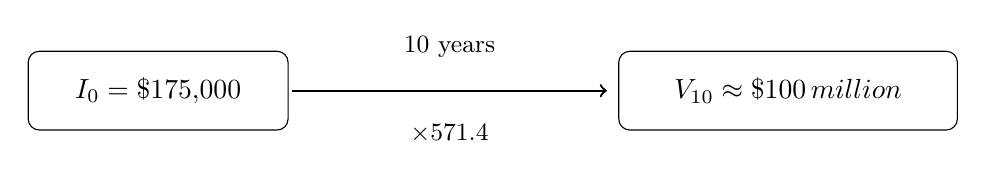
\begin{tikzpicture}[scale=1]
\node[draw, rounded corners, minimum width=3.3cm, minimum height=1cm] at (0,0) (s) {\(I_0=\$175{,}000\)};
\node[draw, rounded corners, minimum width=4.3cm, minimum height=1cm] at (8,0) (t) {\(V_{10}\approx \$100\,\text{million}\)};
\draw[->, thick] (1.7,0) -- (5.7,0);
\node at (3.7,0.55) {\small \(10\) years};
\node at (3.7,-0.55) {\small \(\times 571.4\)};
\end{tikzpicture}
\caption{Transcript-based reconstruction of the lecture's clearest quantitative story. The entrepreneur compresses a ten-year business history into a start-end transformation from \(\$175{,}000\) to roughly \(\$100\) million.}
\end{figure}

\subsection{Question \& Answer}

\paragraph{Question.}
When should we bet everything on ourselves, and when should we switch into preservation mode?

\paragraph{Answer.}
The lecture's answer is sequential rather than universal. Early in the entrepreneurial phase, if we truly believe we possess an edge, concentration may be rational: the founder bets on the business because the founder is the highest-conviction asset in view. After the large win, however, the logic changes. The goal is no longer maximum concentration of upside. It is preservation, multiplication, and diversification of already accumulated capital. The lecture is therefore not preaching blind self-belief. It is teaching that capital policy changes with stage.

\section{Critics, Customer Recognition, and the Discipline of an Easy Life}

After the numerical compression comes a necessary question: what interior structure allowed that compression to happen? The lecture answers in stages.

\paragraph{Anecdote.}
First comes criticism. She says that of course a very successful woman has attracted hate. Her answer is not therapeutic. It is functional. The people with the most to say are usually the ones sitting on the sidelines rather than doing the work. They are in the bleachers, not in the game.

\paragraph{Claim.}
This is a doctrine about authority. Commentary from non-builders has low informational value.

\paragraph{Mechanism.}
The lecture then shifts from critics to customer experience through Dale Carnegie. She names \emph{How to Win Friends and Influence People}, and from it extracts an operational rule: use the customer's name. At Solidcore, hearing one's own name again and again makes one feel seen, respected, and at home. The structure is easy to summarize:
\begin{equation}
\text{name recognition}
\to
\text{felt respect}
\to
\text{return behavior}.
\end{equation}
This is one of the more elegant moves in the lecture. A soft interpersonal point becomes a retention mechanism.

Then the lecture pivots once more, this time into discipline. She gives the aphorism
\begin{equation}
\text{easy choices} \to \text{hard life},
\qquad
\text{hard choices} \to \text{easy life},
\end{equation}
and immediately refuses to leave it as slogan. She grounds it in a schedule:
\begin{equation}
t_{\text{wake}} \approx 5{:}30\text{--}6{:}00\ \text{a.m.},
\qquad
d_{\text{gym}} = 6/\text{week},
\end{equation}
\begin{equation}
h_{\text{volleyball}} \approx 2\text{--}3\ \text{hours/day},
\qquad
d_{\text{volleyball}} = 5/\text{week}.
\end{equation}
From this we can compute the weekly volleyball load:
\begin{equation}
H_{\text{volleyball}}
=
h_{\text{volleyball}}\,d_{\text{volleyball}}
\approx
10\text{--}15\ \text{hours/week}.
\end{equation}
That is not decorative exercise. It is evidence that the lecture's moral vocabulary is backed by operating structure.

\subsection{Question \& Answer}

\paragraph{Question.}
Why do hard choices feel punishing now but protective later?

\paragraph{Answer.}
Because the lecture frames discipline as intertemporal trade. The easy action gives immediate comfort but weakens the future self; the hard action burdens the present self but strengthens the future one. What matters here is that the lecture does not merely say this. It exhibits the principle as repeated, measurable behavior: wake time, gym days, sport hours, food discipline, and the refusal to put oneself into obviously degrading situations.

The host then asks whether building a \(\$100\) million company was worth the sacrifice. Her answer is subtle. She says it did not feel like sacrifice because she loved the work, loved the team, and believed the company was making people stronger. We should keep that beat. It prevents the lecture from collapsing into a purely stoic account of suffering. Purpose changes the felt cost of effort.

The sponsor-community interlude that follows adds no mathematical content, but it does perform an important rhythmic function. It cools the room, breaks the density of doctrine, and resets the episode for the final long-duration founder case.

\section{The Yacht-Side Beauty Founder: One Bottle, Fifteen Companies, and Strategic Differentiation}

The last major movement returns us to the marina. At first it looks as though the lecture is returning to pure luxury spectacle, but in fact it is about duration, restart, and ownership.

The founder says she has been in the beauty industry for forty-two years and that she now has fifteen companies:
\begin{equation}
t_{\text{beauty}} = 42\ \text{years},
\qquad
N_{\text{companies}} = 15.
\end{equation}
When asked for the most made in a single year, the answer is ``nine figures,'' so the safest mathematical form is
\begin{equation}
Y_{\text{hair}} \ge \$100\,\text{million}.
\end{equation}

\paragraph{Anecdote.}
But the lecture immediately pulls downward in scale. Her first business was no grand enterprise, only a tiny square of working space in which she did hair. Later, an entire company failed. She lost everything. Then came the restart, and it began with a single bottle, because nothing more could be afforded.

\paragraph{Claim.}
The lecture's claim here is that scale is often built twice: once in fantasy and once again after failure, when the vanity has been burned out of it.

\paragraph{Mechanism.}
The key transition is ownership. She says she spent ten years in the business with a partner and then bought the partner out. The final result is full founder control:
\begin{equation}
f_{\text{founder}} = 100\%.
\end{equation}
The whole path can be schematized as
\begin{equation}
\text{failed first company}
\to
\text{restart with one bottle}
\to
\text{buy out partner}
\to
100\% \text{ founder-owned global brand}.
\end{equation}

The lecture then gives one of its best tests for real brand power. She tells the airport story: she walks into a salon, asks whether they carry her product, and learns that they have just sold the last bottle and are carrying it despite pressure from another brand. This is not merely flattering anecdote. It is market evidence. The brand has crossed from founder intention into customer pull.

\subsection{Question \& Answer}

\paragraph{Question.}
How do we know that a brand has crossed from founder hope into real market pull?

\paragraph{Answer.}
The lecture's answer is not abstract. We know it when the product moves without pleading, when others carry it because demand forces their hand, and when customers feel enough attachment to it that the founder can discover the brand already alive in someone else's voice. That is why the airport story matters. It is the lecture's cleanest anecdotal test of organic demand.

The closing advice then becomes strategic rather than motivational. It is not what we have but what we do with what we have. It is not even merely about working harder. It is about being smarter, more strategic, going where others do not go, and zigging when they zag:
\begin{equation}
\text{crowded path} \to \text{differentiation},
\qquad
\text{zig when they zag}.
\end{equation}
That is how the lecture ends: not with a mystical personality trait, but with a rule of asymmetry.

\section{Summary}

This lecture begins with objects and ends with structures. First the yacht, the G-Wagon, the Bentley, the exit value, and the billionaire label; then the mechanisms beneath them: selling, borrowing, spreading capital, network reserve, tax-team architecture, concentrated self-betting, later diversification, customer recognition, disciplined intertemporal trade, restart after failure, partner buyout, and strategic differentiation. The clearest mathematical spine lies in the Solidcore compression
\[
\$175{,}000 \to \$100\,\text{million in 10 years},
\]
but the larger lesson is broader than that one transformation. Wealth in this lecture is never finally explained by glamour. It is explained by sequence, by stage, by operating structure, and by the ability to rebuild when the first version of the machine breaks.